\chapter{Konzept}
    Wie in der Einleitung bereits erwähnt, stellt die begrenzte Bandbreite beim autonomen Fahren eine Herausforderung dar, da die enormen Datenmengen die verfügbaren Ressourcen schnell überlasten. Eine mögliche Lösung besteht darin, die Bilder zu verkleinern, bevor sie in die Cloud hochgeladen werden.
    
    Ziel dieser Arbeit ist es, Originalbilder, Bilder mit nicht KI-basierter Kompression im verlustbehafteten Format JPEG sowie Bilder, die mit KI-basierter Kompression reduziert und anschließend rekonstruiert wurden, miteinander zu vergleichen. Dabei sollen Rückschlüsse und Erkenntnisse über die Qualität der Bilder im Vergleich zu den Originalbildern sowie untereinander gewonnen werden. Zusätzlich sollen mögliche Zusammenhänge, Abhängigkeiten oder Kausalitäten identifiziert werden.
    Dies wird mithilfe der bereits vorgestellten Metriken durchgeführt, um die Bildqualität in Abhängigkeit von der Art und Intensität der Kompression zu bewerten.
    Zunächst muss für die Aufgabendomäne des autonomen Fahrens ein passender Datensatz ausgewählt werden. Schließlich sollen reale, domänenspezifische Daten verwendet werden. Geeignet hierfür sind Datensätze wie KITTI, CamVid und Cityscapes. In dieser Arbeit wurde der Datensatz Cityscapes gewählt, da er besonders hochauflösende Bilder aus realen Straßenszenen im Straßenverkehr enthält.

    \begin{figure}[!htb]
        \centering
        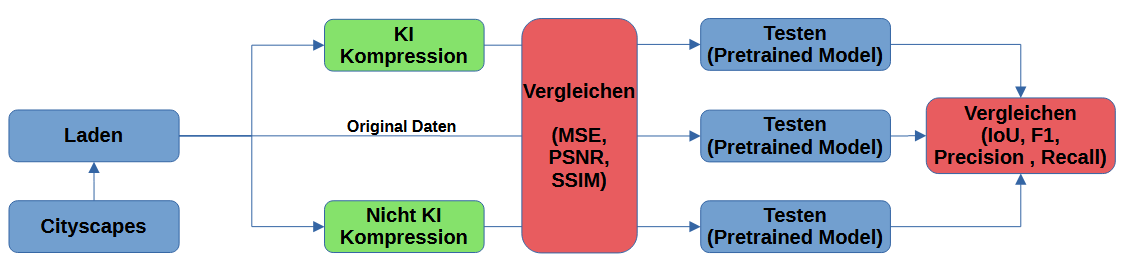
\includegraphics[scale=0.49]{pictures/PAP_2.0.png}
        \caption{PAP Diagramm welches das Vorgehen dieser Arbeit veranschaulicht.}
    \end{figure}
    
    Zunächst wird der Cityscapes-Datensatz zweimal dupliziert und aufgeteilt. Ein Datensatz wird in ein VQ-VAE-Modell eingespeist, wodurch die KI-komprimierten und rekonstruierten Daten erzeugt werden. Der andere Datensatz wird mit einem nicht-KI-basierten Verfahren komprimiert, wobei hier JPEG, ein verlustbehaftetes Bildformat, verwendet wird. So entstehen neben dem Originaldatensatz auch KI-rekonstruktierte Daten sowie JPEG-komprimierte Daten.
    
    Die JPEG-komprimierten Daten sowie die durch KI erzeugten Daten werden mit den Originaldaten abgeglichen und verglichen. Die Metriken, die in diesem Schritt verwendet werden, um Rückschlüsse zu ziehen, sind MSE, PSNR und SSIM.
    Diese Metriken geben Aufschluss über die Qualität der Bilder im Vergleich zu ihrem Original.
    Es gibt verschiedene Kompressionsstufen, die unterschiedliche Ergebnisse liefern, wenn sie auf ihre Qualität untersucht werden. So werden die KI-erzeugten und die JPEG-Daten ebenfalls hinsichtlich ihrer Qualität in Abhängigkeit von der Kompressionsstufe untersucht.
    Im nächsten Schritt werden die drei Datensätze in ein Modell eingegeben, das auf den Bildern Objekte detektiert und Boundingboxen um diese legt. Der Originaldatensatz dient dabei als Label und enthält die Ground-Truth-Boundingboxen.
    Es wird erneut verglichen, wie die KI-generierten Daten und die JPEG-Daten im Vergleich zu den Ground-Truth-Daten abschneiden. Hierfür werden Metriken wie Precision, Recall und F1-Score verwendet sowie der IoU (Intersection over Union), um zu untersuchen, wie gut Vorhersagen getroffen werden. 
    Ob in den Boundingboxen der Labels tatsächlich das richtige Objekt zu erkennen ist oder nicht, spielt keine Rolle. Sie dienen als Ground-Truth-Boundingboxen, anhand derer die rekonstruierten und komprimierten Bilder gemessen werden, die versuchen müssen, diese so gut wie möglich zu approximieren.